\documentclass[]{article}

\usepackage[english]{babel}
\usepackage{graphicx}
\usepackage{booktabs}
\usepackage{float}
\usepackage{hyperref}

\title{Recurrent Neural Networks}
\author{Juan Lao Tebar}

\begin{document}
	
	\maketitle
	
	\section{Introduction} 

	In this practice we explore the effects of the different elements of RNNs using a specific dataset\footnote{\url{https://upc-mai-dl.github.io/rnn-lab-autonomous/}} by extending the Wind prediction example of the previous guided session.
	
	In the original example we predicted one step of the future wind---next 15 minutes---using a window of previous measurements. Here we extend the problem in different ways:
	
	\begin{description}
		\item [Complementary variables.] In the original experiment we used only the wind speed as input data. Now we include also the air density, the temperature and the pressure.
		
		\item [Complementary sites.] In the original experiment we predicted the wind speed using the data from one site, but the dataset includes three additional sites that are geographically close---they are in the vertices of a 2 km square---. Here we leverage the information of the wind speed from the other sites.
		
		\item [Multi step prediction.] Here we obtain a multi step prediction using the original model simply by adding the value predicted to the current set of measurements and discarding the oldest one.
		
		\item [Sequence to sequence prediction.] An alternative to shifting the input and adding the predictions to have a multi step prediction is a network that links a window of measurements to a window of predictions.
	\end{description}
	
	In this practice we change the stopping criteria of the training process, as we remove the limit of epochs and we implement a stopper based on the validation loss: when we detect a minimum value, we stop the training after 30 epochs if it does not decrease again. If the model does not show any sign of convergence, we consider that we should not stop the training process just because it reached an arbitrary number of epochs.
	
	In the guided laboratory we trained the model with 50,000 samples, validated with 10,000 and tested with 10,000, while in this practice we use the whole dataset, training our model with 122,736 samples, validating with 61,368 and testing with 61,368.
	
	The code related to this work is public and available at github\footnote{\url{https://github.com/juanlao7/DL-lab2}}.
	
	\section{Baseline}
	
	Before performing any experiment, we define a baseline model in order to compare the results and determine how each change affects the accuracy of the system.
	
	Our baseline model is similar to the one proposed in the guided laboratory: an input window size of 6 steps, 1 output, 512 LSTM units in one single hidden layer and no dropout, trained with RMSprop---with a learning rate of 0.0001, $ \rho = 0.9 $, $ \varepsilon = 1 \cdot 10^{-8} $ and no learning rate decay.
	
	Table \ref{t:baseline} shows the results obtained with this model.
	
	\begin{table}[H]
		\centering
		\begin{tabular}{@{}ccc@{}}
			\toprule
			Training loss & Validation loss & Test loss \\ \midrule
			0.02729       & 0.02924         & 0.03339   \\ \bottomrule
		\end{tabular}
		\caption{Results obtained with the baseline model.}
		\label{t:baseline}
	\end{table}
	
	\section{Complementary Variables}
	
	\subsection{Plan}
	
	In this session we modify the architecture of the system adequately for taking all the variables as input---but still giving only one variable as output---. Then we study how the MSE is affected by the size of the hidden layer, the dropout and the size of the input window.
	
	\begin{itemize}
		\item In the 1st experiment we test different layer sizes: 32, 128, 512 and 1024 units.
		
		\item In the 2nd experiment we test different dropout factors applied in the LSTM layer, including its gates: 0\%, 25\%, 50\%, 75\%.
		
		\item In the 3rd experiment we test different dropout factors only applied on inter-layer connections, between the hidden and the output layer: 0\%, 25\%, 50\%, 75\%.
		
		\item In the 4th experiment we test different input window sizes: 1, 3, 6, 12, 24, 48. In this experiment, in the case of the window size of 48, we had to clip all parameter gradients to a maximum norm of 1 in order to prevent exploding gradients.
	\end{itemize}
	
	\subsection{Expectations}
	
	Regarding to the learning techniques:
	
	\begin{itemize}
		\item In theory, adding more units to the hidden layer leads to better training accuracies. However, the model may lose power of generalization, overfitting the training data and offering worse validation and test accuracies.
		
		\item If the network overfits the training data, we expect that applying a dropout factor will successfully regularize the model. However, the dropout implementation we use---``dropout'' argument in Keras implementation of LSTM layers---affects also to the LSTM gates, thus it is possible that the model will end up performing even worse due to the vanishing gradient problem. For this reason we also test an inter-layer dropout, that does not affect to LSTM gates. On the other hand, if the model does not overfit, dropout will slightly reduce the gap between training and validation losses, but not in a considerable way.
		
		\item We suspect that in this dataset there are no data relations over long intervals of time, hence we will not obtain a better result by increasing the window size. However, decreasing it may lead to a worse accuracy.
	\end{itemize}
	
	Regarding to this specific problem:
	
	\begin{itemize}
		\item More information---variables---are always helpful and the model may find new inter-variable relations that lead to a better accuracy.
	\end{itemize}
	
	\subsection{Results}
	
	\begin{itemize}
		\item Table \ref{t:variables_1} shows the results obtained after testing different layer sizes, while figure \ref{f:variables_1} shows the evolution of the training and validation loss in each case.
		
		\item Table \ref{t:variables_2} shows the results obtained after testing different dropout factors, while figure \ref{f:variables_2} shows the evolution of the training and validation loss in each case.
		
		\item Table \ref{t:variables_3} shows the results obtained after testing different inter-layer dropout factors, while figure \ref{f:variables_3} shows the evolution of the training and validation loss in each case.
		
		\item Table \ref{t:variables_4} shows the results obtained after testing different input window sizes, while figures \ref{f:variables_4_1} and \ref{f:variables_4_2} show the evolution of the training and validation loss in each case.
	\end{itemize}
	
	\begin{table}[H]
		\centering
		\begin{tabular}{@{}cccc@{}}
			\toprule
			& Training loss & Validation loss & Test loss \\ \midrule
			32 LSTM units   & 0.02770       & 0.02939         & 0.03327   \\
			128 LSTM units  & 0.02621       & 0.02835         & 0.03218   \\
			512 LSTM units  & 0.02562       & 0.02911         & 0.03266   \\
			1024 LSTM units & 0.02531       & 0.02883         & 0.03247   \\ \bottomrule
		\end{tabular}
		\caption{Results obtained after testing different layer sizes.}
		\label{t:variables_1}
	\end{table}
	
	\begin{figure}[H]
		\centering
		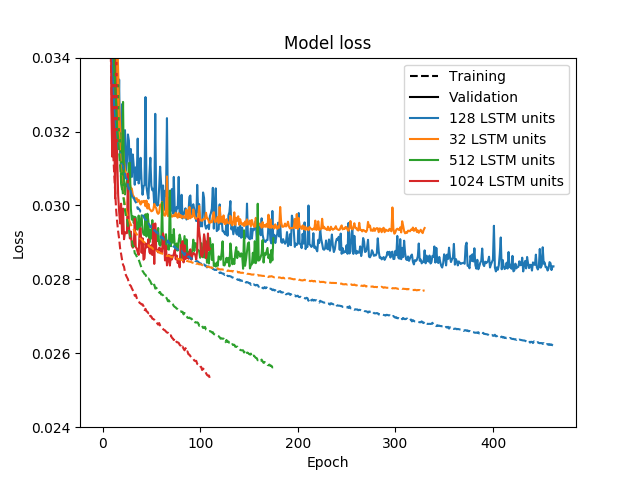
\includegraphics[width=0.5\textwidth]{variables_1}
		\caption{Validation and training loss with each layer size.}
		\label{f:variables_1}
	\end{figure}
	
	\begin{table}[H]
		\centering
		\begin{tabular}{@{}cccc@{}}
			\toprule
			& Training loss & Validation loss & Test loss \\ \midrule
			0\% dropout  & 0.02562       & 0.02911         & 0.03266   \\
			25\% dropout & 0.24172       & 0.08519         & 0.08502   \\
			50\% dropout & 0.47773       & 0.27423         & 0.26216   \\
			75\% dropout & 0.73191       & 0.57920         & 0.54833   \\ \bottomrule
		\end{tabular}
		\caption{Results obtained after testing different dropout factors.}
		\label{t:variables_2}
	\end{table}
	
	\begin{figure}[H]
		\centering
		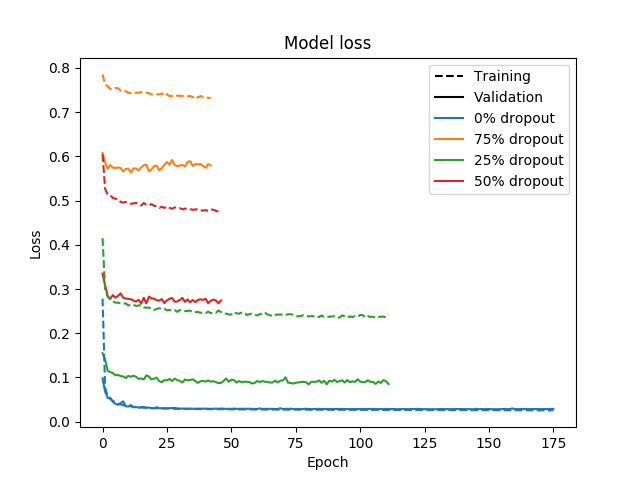
\includegraphics[width=0.5\textwidth]{variables_2}
		\caption{Validation and training loss with each dropout factor.}
		\label{f:variables_2}
	\end{figure}
	
	\begin{table}[H]
		\centering
		\begin{tabular}{@{}cccc@{}}
			\toprule
			& Training loss & Validation loss & Test loss \\ \midrule
			0\% inter-layer dropout  & 0.02562       & 0.02911         & 0.03266   \\
			25\% inter-layer dropout & 0.02830       & 0.02886         & 0.03258   \\
			50\% inter-layer dropout & 0.03110       & 0.02884         & 0.03262   \\
			75\% inter-layer dropout & 0.04012       & 0.02975         & 0.03337   \\ \bottomrule
		\end{tabular}
		\caption{Results obtained after testing different inter-layer dropout factors.}
		\label{t:variables_3}
	\end{table}
	
	\begin{figure}[H]
		\centering
		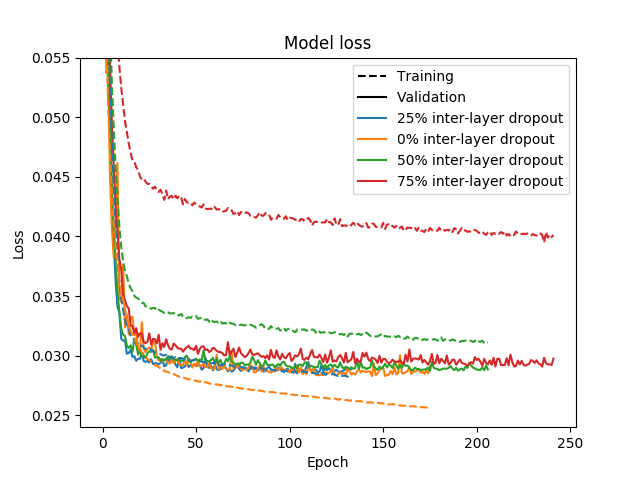
\includegraphics[width=0.5\textwidth]{variables_3}
		\caption{Validation and training loss with each inter-layer dropout factor.}
		\label{f:variables_3}
	\end{figure}
	
	\begin{table}[H]
		\centering
		\begin{tabular}{@{}cccc@{}}
			\toprule
			& Training loss & Validation loss & Test loss \\ \midrule
			Window size of 1  & 0.03146       & 0.03305         & 0.03599   \\
			Window size of 3  & 0.02690       & 0.02880         & 0.03254   \\
			Window size of 6  & 0.02562       & 0.02911         & 0.03266   \\
			Window size of 12 & 0.02586       & 0.02884         & 0.03260   \\
			Window size of 24 & 0.02465       & 0.02941         & 0.03375   \\
			Window size of 48 & 0.02543       & 0.02885         & 0.03316   \\ \bottomrule
		\end{tabular}
		\caption{Results obtained after testing different input window sizes.}
		\label{t:variables_4}
	\end{table}
	
	\begin{figure}[H]
		\centering
		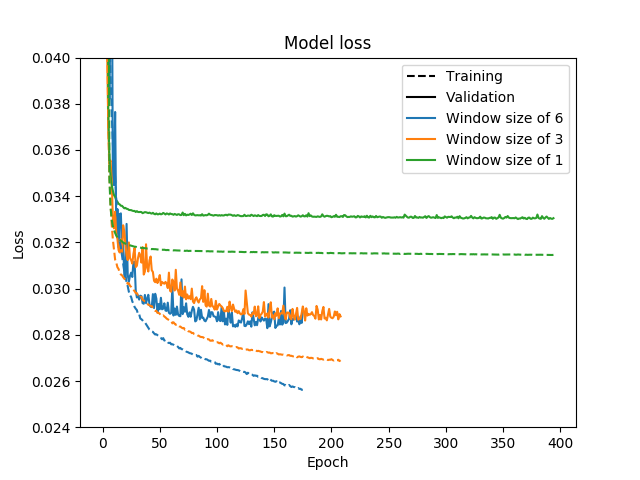
\includegraphics[width=0.5\textwidth]{variables_4_1}
		\caption{Validation and training loss with window sizes 1, 3 and 6.}
		\label{f:variables_4_1}
	\end{figure}
	
	\begin{figure}[H]
		\centering
		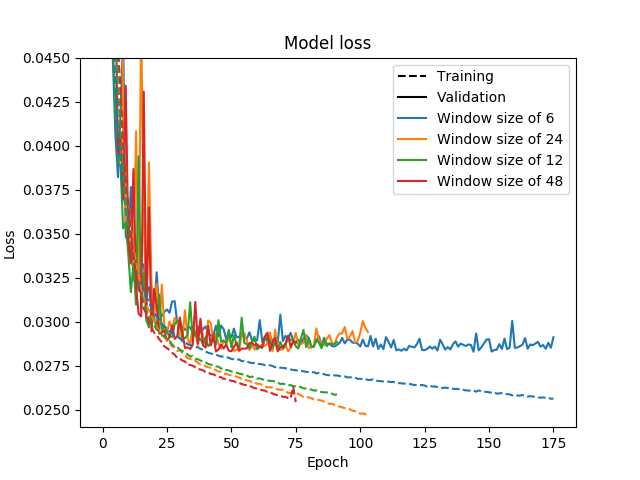
\includegraphics[width=0.5\textwidth]{variables_4_2}
		\caption{Validation and training loss with window sizes 6, 12, 24 and 48.}
		\label{f:variables_4_2}
	\end{figure}
	
	\subsection{Conclusions}
	
	Regarding to the learning techniques:
	
	\begin{itemize}
		\item \emph{As expected}, adding more units to the hidden layer leads to better training accuracies and, for the case of 1024 units, overfits the training data and offers worse validation and test accuracies.
		
		\item \emph{As expected}, dropout factors applied to LSTM gates lead to far worse results than the original approach.
		
		\item \emph{As expected}, since our model does not overfit the training data, certain dropout factors---25\% in this case---reduce the gap between the training and validation loss, but does not increase the accuracy of the system.
		
		\item \emph{As expected}, smaller window sizes lead to worse accuracies while bigger window sizes do not offer much improvement. However, it seems that the model converges in a lesser number of epochs.
	\end{itemize}
	
	Regarding to this specific problem:
	
	\begin{itemize}
		\item \emph{As expected}, more information---variables---are helpful and the model finds new inter-variable relations that lead to a \emph{slightly} better accuracy. The baseline model got a test accuracy of 0.03339 while our best model here got 0.03218---and several configurations got a mark under 0.03290---. We conclude that air density, pressure and temperature help to predict wind speed at 100m in site ``90-45142''.
	\end{itemize}
	
	\section{Complementary Sites}
	
	\subsection{Plan}
	
	In this session we leverage the information of the wind speed from other sites and we study how the MSE is affected by the size of the hidden layer, the dropout and the size of the input window.
	
	\begin{itemize}
		\item In the 1st experiment we test different layer sizes: 32, 128, 512 and 1024 units.
		
		\item In the 2nd experiment we test different dropout factors applied in the LSTM layer, including its gates: 0\%, 25\%, 50\%, 75\%.
		
		\item In the 3rd experiment we test different dropout factors only applied on inter-layer connections, between the hidden and the output layer: 0\%, 25\%, 50\%, 75\%.
		
		\item In the 4th experiment we test different input window sizes: 1, 3, 6, 12, 24, 48. In this experiment, in the case of the window size of 48, we had to clip all parameter gradients to a maximum norm of 1 in order to prevent exploding gradients.
	\end{itemize}
	
	\subsection{Expectations}
	
	Exactly the same as in Complementary Variables.
	
	\subsection{Results}
	
	\begin{itemize}
		\item Table \ref{t:sites_1} shows the results obtained after testing different layer sizes, while figure \ref{f:sites_1} shows the evolution of the training and validation loss in each case.
		
		\item Table \ref{t:sites_2} shows the results obtained after testing different dropout factors, while figure \ref{f:sites_2} shows the evolution of the training and validation loss in each case.
		
		\item Table \ref{t:sites_3} shows the results obtained after testing different inter-layer dropout factors, while figure \ref{f:sites_3} shows the evolution of the training and validation loss in each case.
		
		\item Table \ref{t:sites_4} shows the results obtained after testing different input window sizes, while figures \ref{f:sites_4_1} and \ref{f:sites_4_2} show the evolution of the training and validation loss in each case.
	\end{itemize}
	
	\begin{table}[H]
		\centering
		\begin{tabular}{@{}cccc@{}}
			\toprule
			& Training loss & Validation loss & Test loss \\ \midrule
			32 LSTM units   & 0.02666       & 0.02821         & 0.03231   \\
			128 LSTM units  & 0.02694       & 0.02855         & 0.03246   \\
			512 LSTM units  & 0.02631       & 0.02847         & 0.03225   \\
			1024 LSTM units & 0.02591       & 0.02882         & 0.03242   \\ \bottomrule
		\end{tabular}
		\caption{Results obtained after testing different layer sizes.}
		\label{t:sites_1}
	\end{table}
	
	\begin{figure}[H]
		\centering
		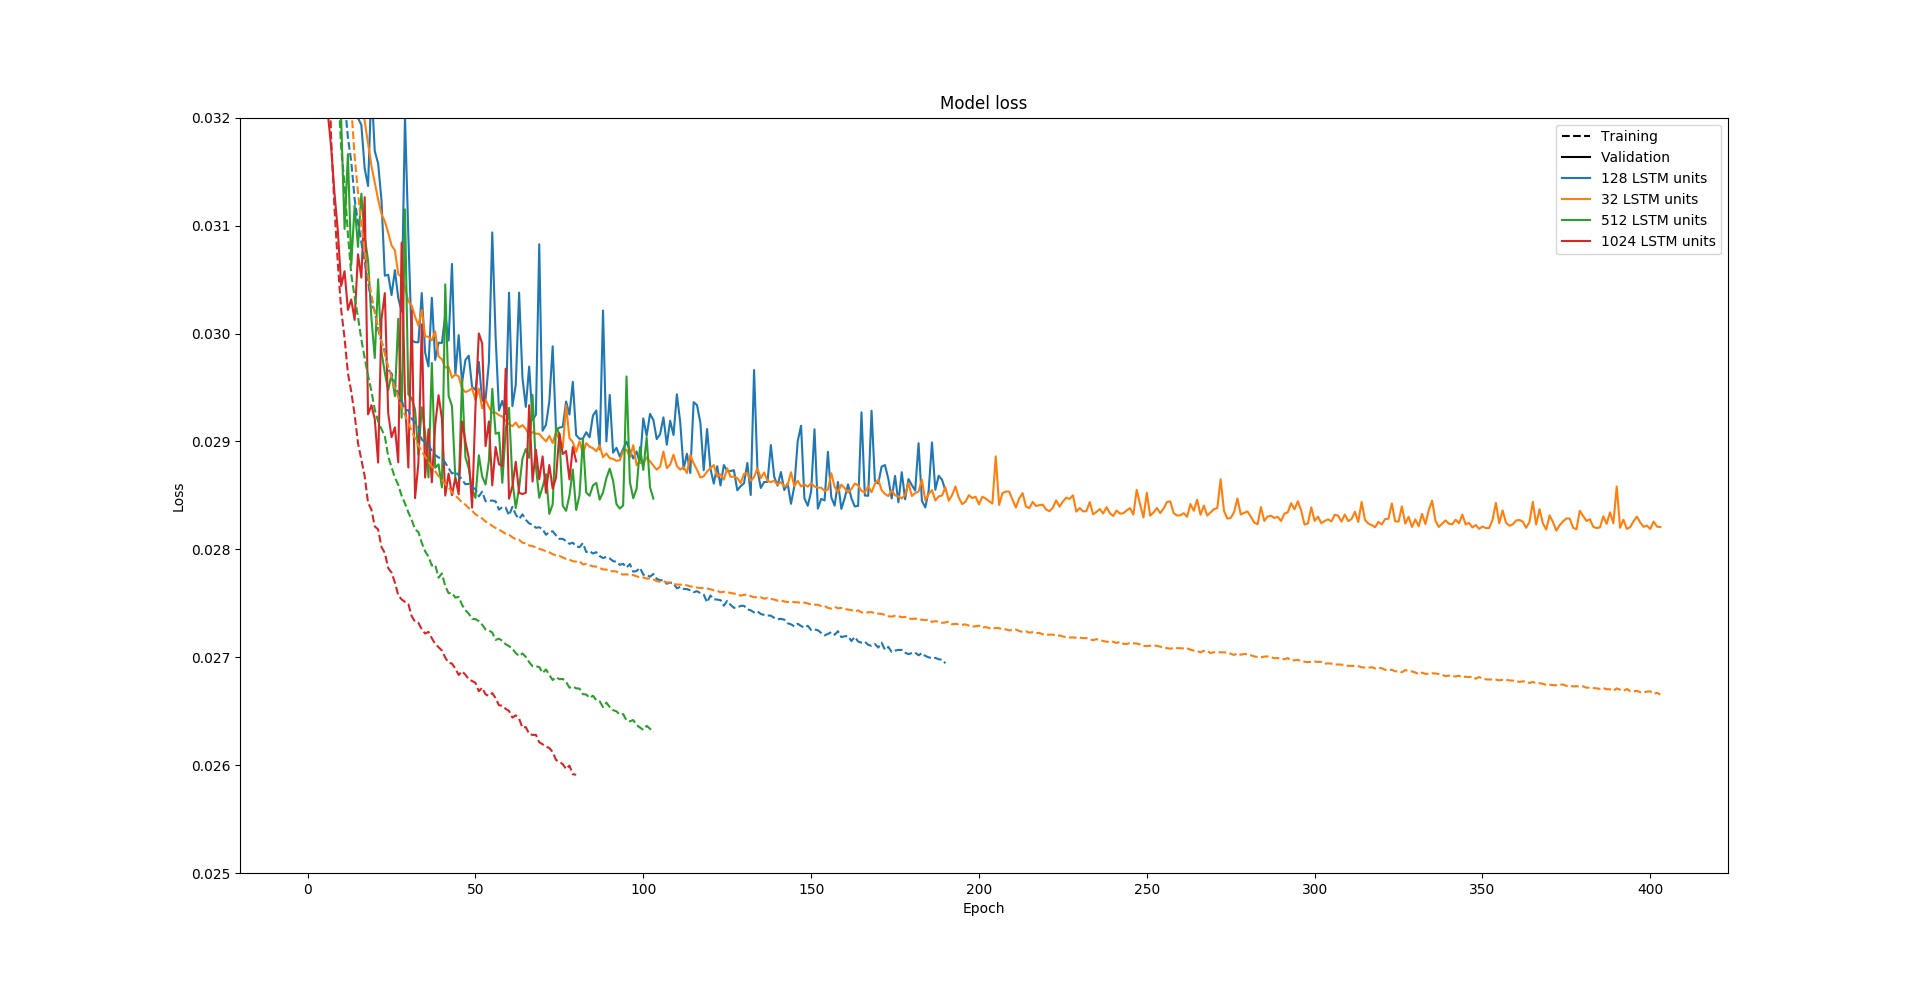
\includegraphics[width=\textwidth]{sites_1}
		\caption{Validation and training loss with each layer size.}
		\label{f:sites_1}
	\end{figure}
	
	\begin{table}[H]
		\centering
		\begin{tabular}{@{}cccc@{}}
			\toprule
			& Training loss & Validation loss & Test loss \\ \midrule
			0\% dropout  & 0.02631       & 0.02847         & 0.03225   \\
			25\% dropout & 0.03554       & 0.08211         & 0.08097   \\
			50\% dropout & 0.09668       & 0.26654         & 0.25337   \\
			75\% dropout & 0.34805       & 0.54228         & 0.51081   \\ \bottomrule
		\end{tabular}
		\caption{Results obtained after testing different dropout factors.}
		\label{t:sites_2}
	\end{table}
	
	\begin{figure}[H]
		\centering
		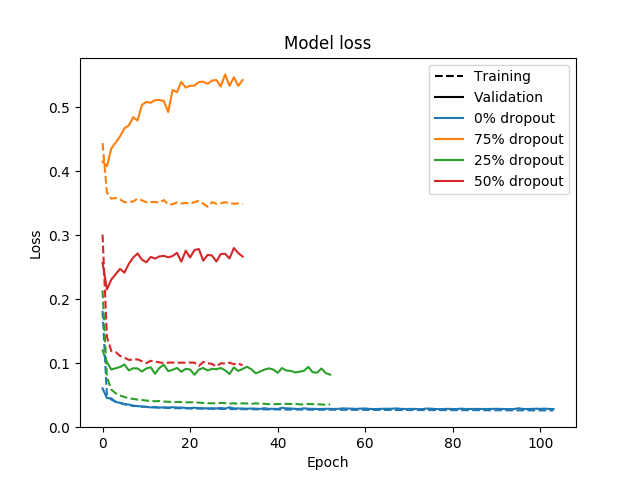
\includegraphics[width=0.5\textwidth]{sites_2}
		\caption{Validation and training loss with each dropout factor.}
		\label{f:sites_2}
	\end{figure}
	
	\begin{table}[H]
		\centering
		\begin{tabular}{@{}cccc@{}}
			\toprule
			& Training loss & Validation loss & Test loss \\ \midrule
			0\% inter-layer dropout  & 0.02631       & 0.02847         & 0.03225   \\
			25\% inter-layer dropout & 0.02836       & 0.02887         & 0.03240   \\
			50\% inter-layer dropout & 0.03084       & 0.02876         & 0.03277   \\
			75\% inter-layer dropout & 0.03898       & 0.02872         & 0.03251   \\ \bottomrule
		\end{tabular}
		\caption{Results obtained after testing different inter-layer dropout factors.}
		\label{t:sites_3}
	\end{table}
	
	\begin{figure}[H]
		\centering
		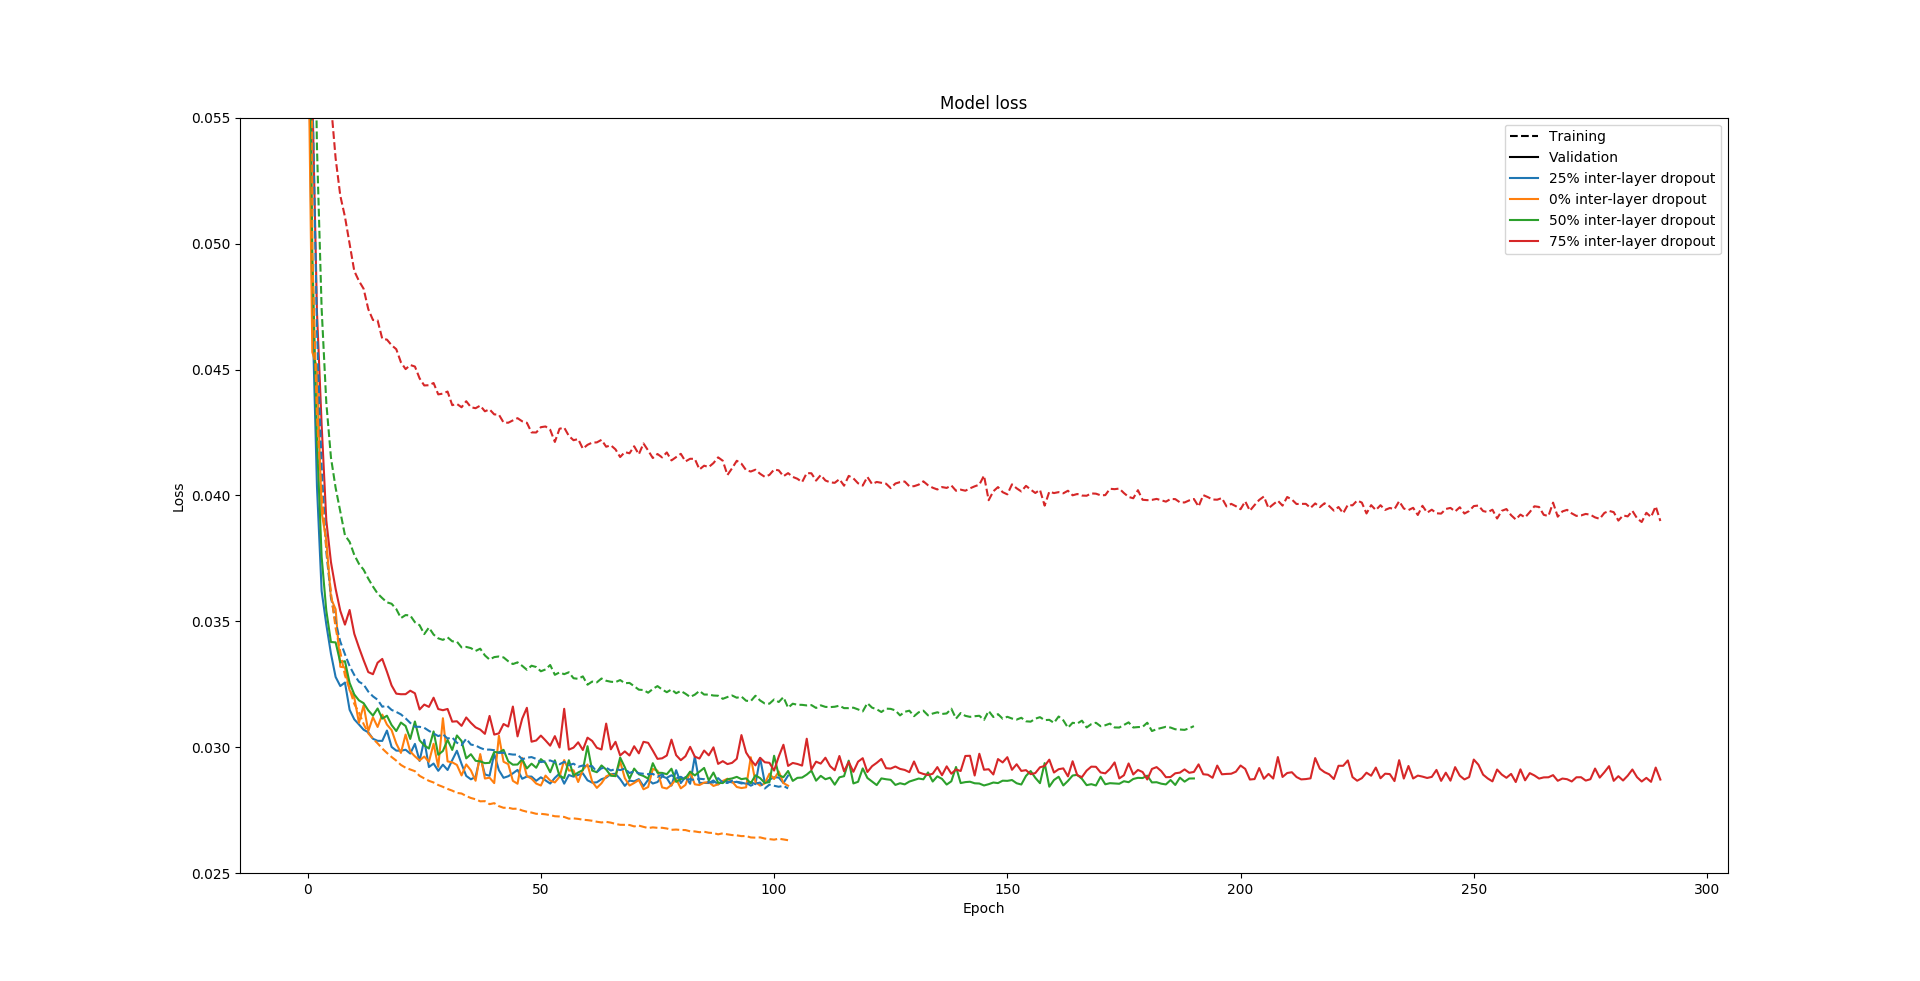
\includegraphics[width=\textwidth]{sites_3}
		\caption{Validation and training loss with each inter-layer dropout factor.}
		\label{f:sites_3}
	\end{figure}
	
	\begin{table}[H]
		\centering
		\begin{tabular}{@{}cccc@{}}
			\toprule
			& Training loss & Validation loss & Test loss \\ \midrule
			Window size of 1  & 0.03136       & 0.03277         & 0.03559   \\
			Window size of 3  & 0.02669       & 0.02843         & 0.03226   \\
			Window size of 6  & 0.02631       & 0.02847         & 0.03225   \\
			Window size of 12 & 0.02558       & 0.02935         & 0.03302   \\
			Window size of 24 & 0.02571       & 0.02879         & 0.03264   \\ \bottomrule
		\end{tabular}
		\caption{Results obtained after testing different input window sizes.}
		\label{t:sites_4}
	\end{table}
	
	\begin{figure}[H]
		\centering
		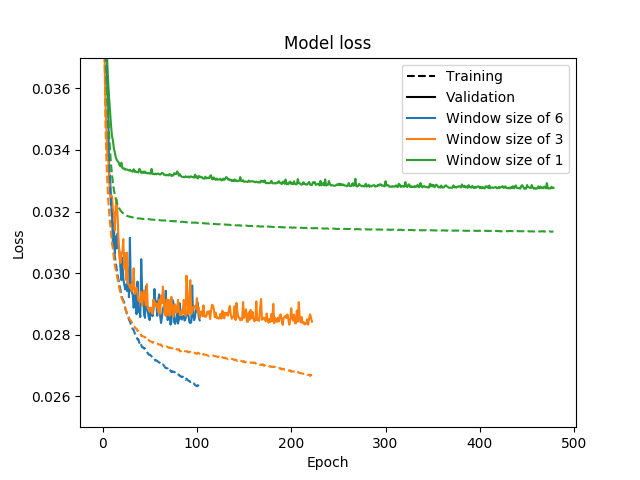
\includegraphics[width=0.5\textwidth]{sites_4_1}
		\caption{Validation and training loss with window sizes 1, 3 and 6.}
		\label{f:sites_4_1}
	\end{figure}
	
	\begin{figure}[H]
		\centering
		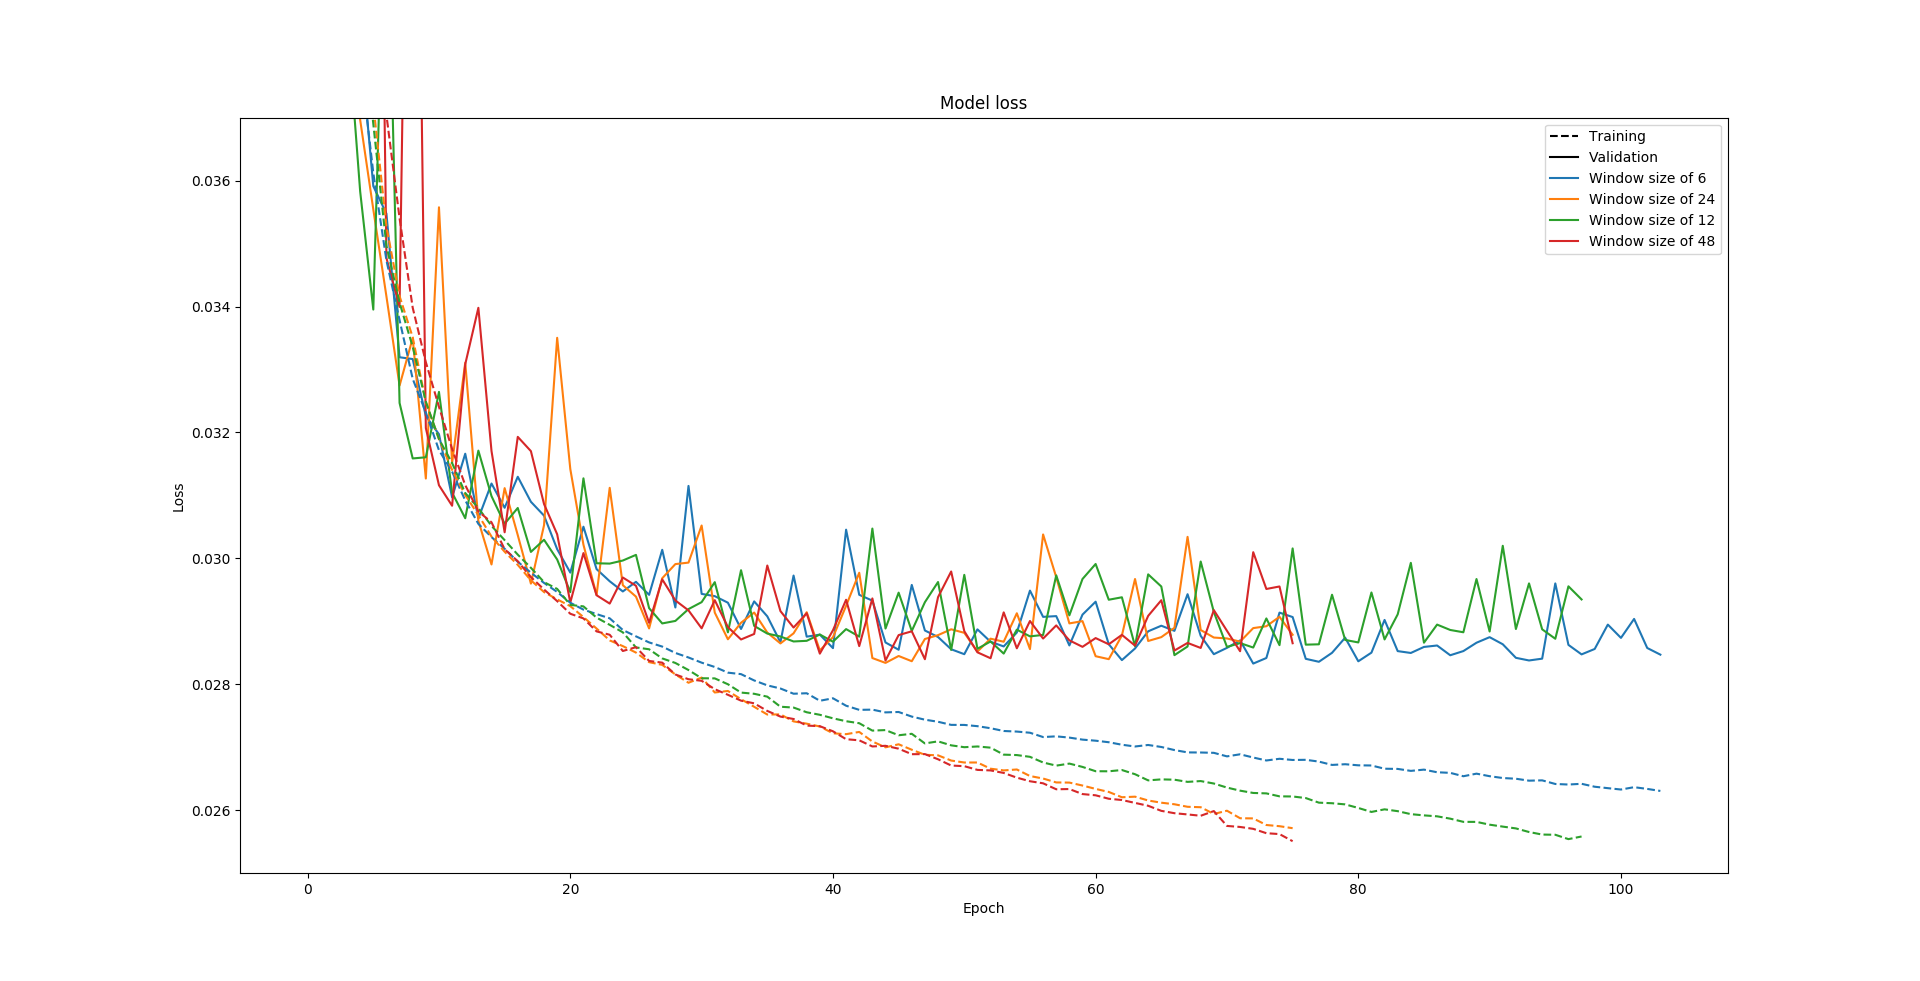
\includegraphics[width=\textwidth]{sites_4_2}
		\caption{Validation and training loss with window sizes 6, 12, 24 and 48.}
		\label{f:sites_4_2}
	\end{figure}
	
	\subsection{Conclusions}
	
	Regarding to the learning techniques: exactly the same as in Complementary Variables.
	
	Regarding to this specific problem:
	
	\begin{itemize}
		\item \emph{As expected}, more information---variables---are helpful and the model finds new inter-variable relations that lead to a \emph{slightly} better accuracy. The baseline model got a test accuracy of 0.03339 while our best model here got 0.03225---and several configurations got a mark under 0.03290---. We can conclude that wind speeds at 100m of sites ``90-45143', ``90-45229'' and ``90-45230'' help to predict wind speed at 100m in site ``90-45142''.
	\end{itemize}
	
	\section{Multi Step Prediction}
	
	\subsection{Plan}
	
	In this session we analyze the behavior of the model when it is fed with its own outputs as new inputs; we study how the MSE degrades the more steps in the future we predict and how the MSE changes if we extend the input window.
	
	In this experiment we test different input window sizes---1, 3, 6, 12, 24---and we observe the evolution of MSE when trying to predict the next 55 steps.
	
	\subsection{Expectations}
	
	\begin{itemize}
		\item In previous experiments we found that small window sizes lead to a higher error, and big window sizes do not show any improvement. We expect that the error of the model accumulates as more steps in the future we predict, leading to a higher error on small window sizes and more stable accuracies in big window sizes.
	\end{itemize}
	
	\subsection{Results}
	
	Figure \ref{f:multistep} shows the results obtained after testing different input window sizes.
	
	\begin{figure}[H]
		\centering
		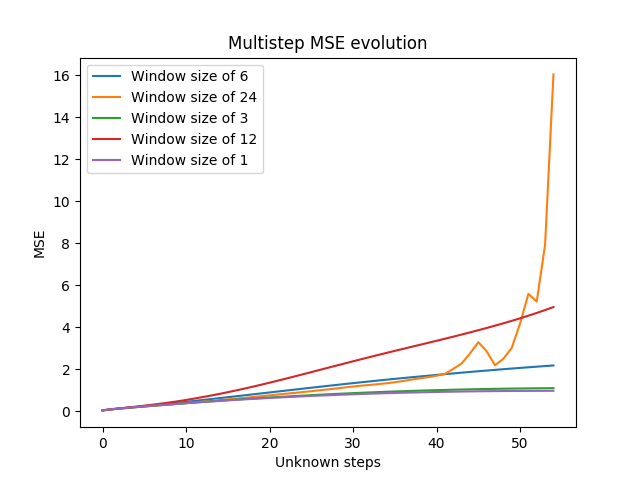
\includegraphics[width=0.5\textwidth]{multistep}
		\caption{MSE evolution for each window size.}
		\label{f:multistep}
	\end{figure}
	
	\subsection{Conclusions}
	
	\begin{itemize}
		\item \emph{Surprisingly}, as we can see in figure \ref{f:multistep}, it turns out that with small window sizes the error seems to converge while in big window sizes the error grows exponentially. Sincerely, we do not have a logical explanation for this interesting phenomena.
	\end{itemize}
	
	\section{Sequence to Sequence Prediction}
	
	\subsection{Plan}
	
	In this session we modify the architecture of the system adequately for linking a window of measurements to a window of predictions, and we study how the MSE of the predictions changes with the length of the predicted sequence.
	
	In this experiment we test different prediction lengths---1, 3, 6, 12, 24---and we observe the evolution of the MSE.
	
	\subsection{Expectations}
	
	\begin{itemize}
		\item Models that try to predict more steps forward will lead to lower accuracies.
		\item This sequence-to-sequence model will have a lower error than the previous multi step approach, since this model does not accumulates the error.
	\end{itemize}
	
	\subsection{Results}
	
	Figure \ref{f:seq2seq_1} shows the evolution of the training and validation loss in each case, while figure \ref{f:seq2seq_2} shows the MSE evolution.
	
	\begin{figure}[H]
		\centering
		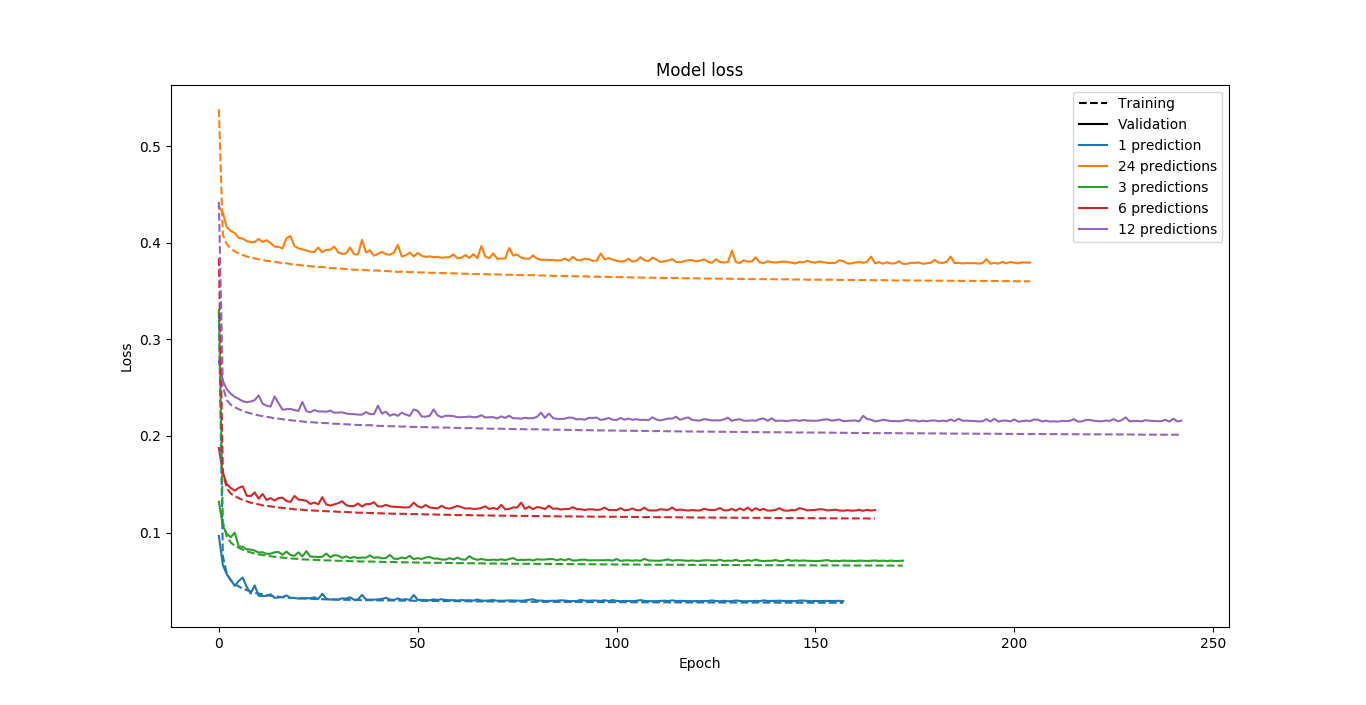
\includegraphics[width=\textwidth]{seq2seq_1}
		\caption{Validation and training loss with each number of predictions.}
		\label{f:seq2seq_1}
	\end{figure}
	
	\begin{figure}[H]
		\centering
		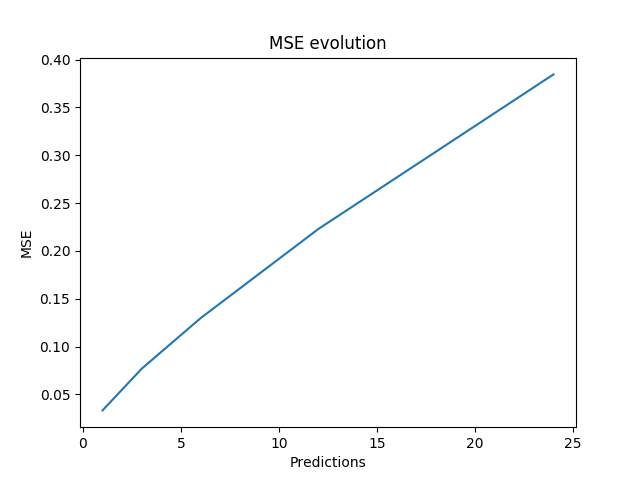
\includegraphics[width=\textwidth]{seq2seq_2}
		\caption{MSE evolution relation with the number of predictions.}
		\label{f:seq2seq_2}
	\end{figure}
	
	\subsection{Conclusions}
	
	\begin{itemize}
		\item \emph{As expected}, models that try to predict more steps forward lead to lower accuracies.
		\item \emph{As expected}, this sequence-to-sequence model has a lower error than the previous multi step approach. The previous model, with a window size of 6 and 24 unknown inputs, has a MSE of 1.06895 while this model has a MSE of 0.368767 when predicting 24 steps.
	\end{itemize}

\end{document}